\section{Data Description}
\label{sec:data-description}
\subsection{Data Sources}
The datasets needed for the exploration of the time series and the fitting of the models have been obtained from the ESIOS -- System Operator's Electronic Information System. This is an online portal where the System Operator, the REE -- Spanish Electrical Grid -- uploads all relevant information for the operation of the grid. 

In order to accomplish everything outlined in \autoref{sec:objective-and-scope} six different datasets are needed. These datasets are:
\begin{itemize}
    \item Real time wind energy hourly generation
    \item Real time solar PV energy hourly generation
    \item Real time solar thermal energy hourly generation
    \item Wind energy monthly installed capacity
    \item Solar PV energy monthly installed capacity
    \item Solar thermal energy monthly installed capacity
\end{itemize}

%\href{https://www.esios.ree.es/es/analisis/551?vis=1&start_date=26-08-2024T00%3A00&end_date=26-08-2024T23%3A55&compare_start_date=25-08-2024T00%3A00&groupby=minutes5}{https://www.esios.ree.es/es/analisis/551}
%\href{https://www.esios.ree.es/es/analisis/1295?vis=1&start_date=26-08-2024T00%3A00&end_date=26-08-2024T23%3A55&compare_start_date=25-08-2024T00%3A00&groupby=minutes5}{https://www.esios.ree.es/es/analisis/1295}
%\href{https://www.esios.ree.es/es/analisis/1294?vis=1&start_date=26-08-2024T00%3A00&end_date=26-08-2024T23%3A55&compare_start_date=25-08-2024T00%3A00&groupby=minutes5}{https://www.esios.ree.es/es/analisis/1294}

\subsection{Data Preprocessing}
The obtained datasets are already very clean, so no missing or obviously wrong values were found on any of them. The installed capacity is obtained on a monthly basis as there is not any lower granularity in the ESIOS portal. With this datasets, the capacity factor is obtained as explained in equation \eqref{eq:capacity-factor} by dividing the generated electricity by the installed capacity times the period time frame. The time frame in this case is always one hour. Like this the hourly capacity factor for the Spanish electrical system for the three different technologies is obtained. Note that the data obtained spans from mid 2015 until end of 2023, since no previous data is available. 

\subsection{Exploratory data analysis}

Now that it is well understood where the data comes from, an initial analysis of the data to understand what the capacity factor of each looks like will be performed. 

\subsubsection{Initial visualization}
The first variable to be visualized will be that of the solar PV capacity factor, which can be seen in 
\begin{figure}[ht]
    \centering
    \captionsetup{justification=centering}
    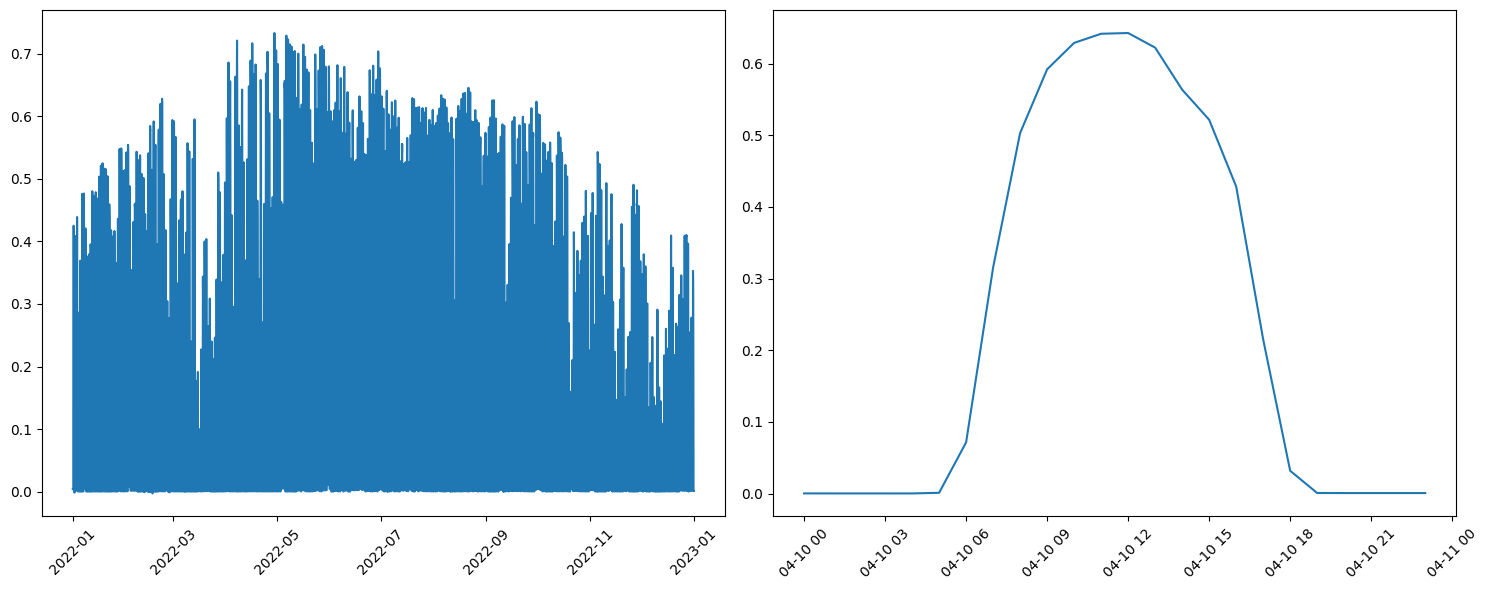
\includegraphics[width=\linewidth]{assets/spv-year-day.png}
    \caption{Yearly and daily profiles of the solar PV capacity factor, taken for 2022 and the 10\textsuperscript{th} April 2022 respectively.}
    \label{fig:spv-year-day}
\end{figure}

The main features of the series can be well visualized here. The yearly seasonality is very clear, with higher peak values in summer and lower peak values in winter, although this is altered by periods of lower sunlight where peaks are reduced below the typical seasonal peak, like at the beginning of March. The daily pattern is also very clear, with values of practically zero -- it is not exactly zero due to some background light and noise in the measurement -- at night and a generation in accordance with the position of the sun in its ecliptic. 

The solar thermal profile, although belonging to the same renewable resource as the solar PV, is slightly different. 
\begin{figure}[ht]
    \centering
    \captionsetup{justification=centering}
    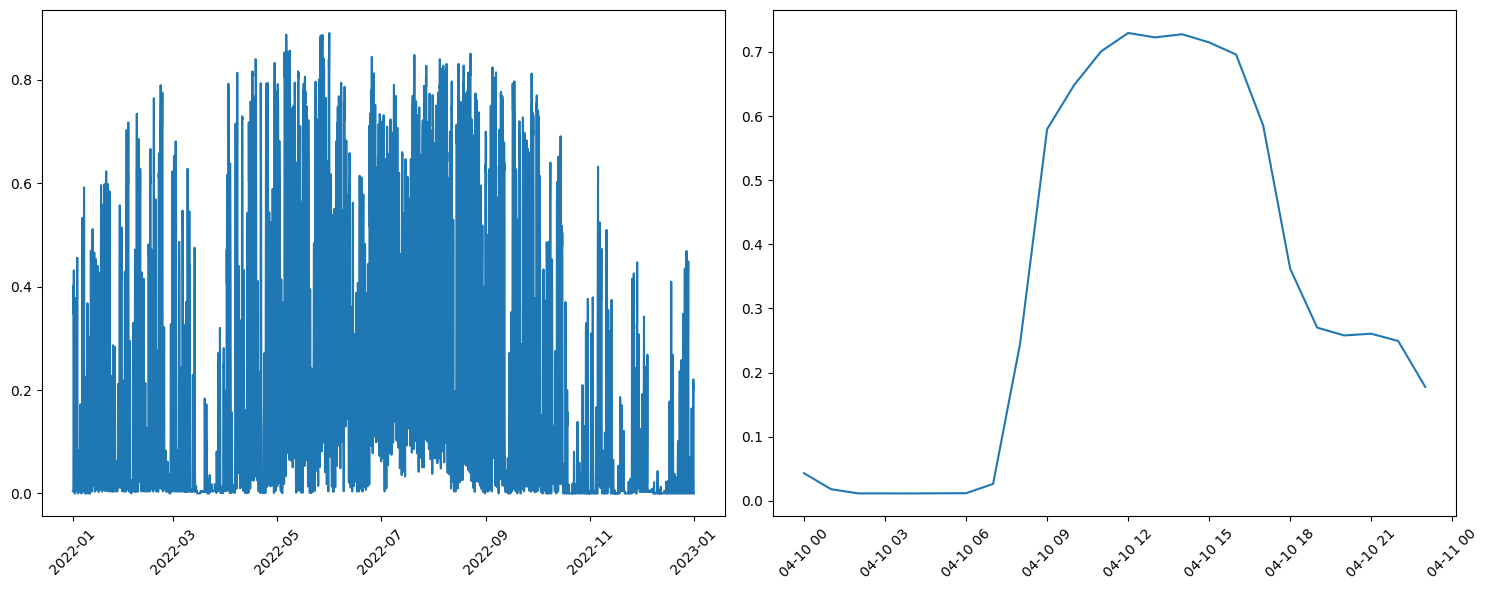
\includegraphics[width=\linewidth]{assets/st-year-day.png}
    \caption{Yearly and daily profiles of the solar thermal capacity factor, taken for 2022 and the 10\textsuperscript{th} April 2022 respectively.}
    \label{fig:st-year-day}
\end{figure}

Several differences between these profiles shown in \autoref{fig:st-year-day} and the previous ones are apparent. The yearly pattern, even though it follows roughly the same seasonality with higher peaks in summer is much more volatile than that of the solar PV. Furthermore, there are whole periods of several days where generation does not go to zero, due to the inertia of the thermal system. The highest peaks are also whigher for the solar thermal, reaching generation values much closer to its rated capacity in the summer than the solar PV. In the daily pattern the mentioned inertia can be clearly seen, where appart from the general sinusoidal throughout the day it can be seen how generation remains above zero at night.

\begin{figure}[ht]
    \centering
    \captionsetup{justification=centering}
    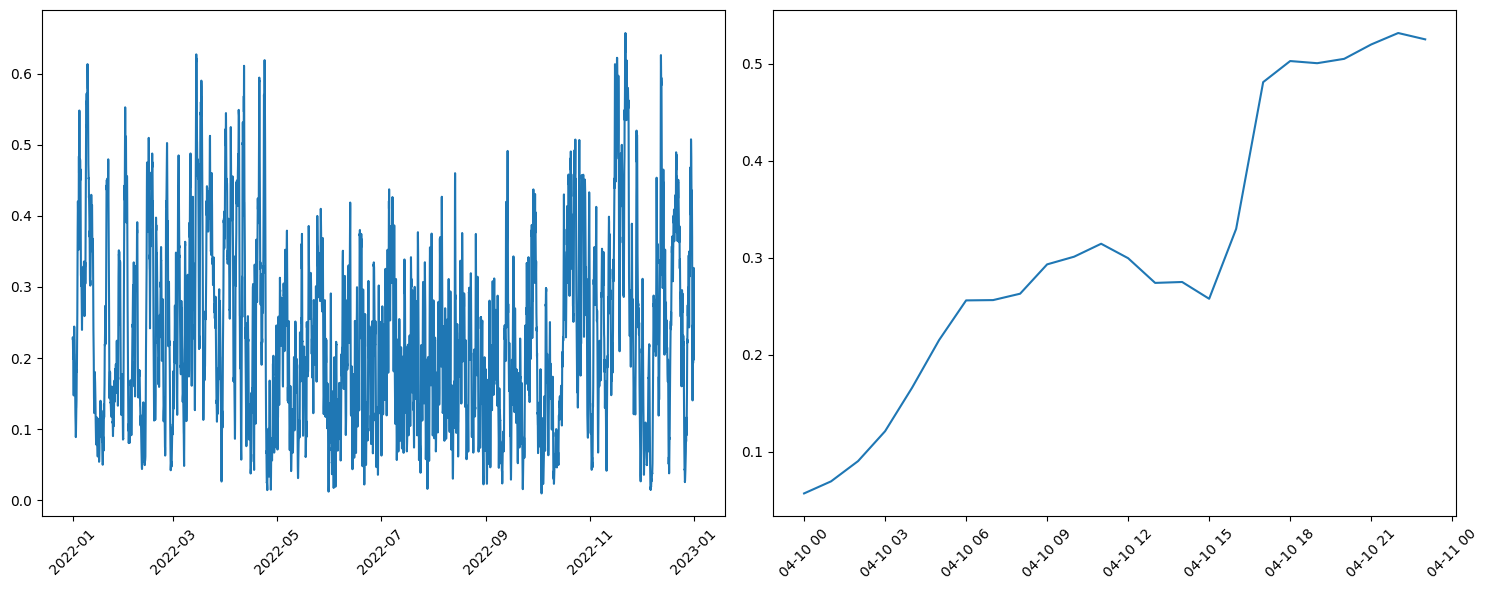
\includegraphics[width=\linewidth]{assets/w-year-day.png}
    \caption{Yearly and daily profiles of the wind capacity factor, taken for 2022 and the 10\textsuperscript{th} April 2022 respectively.}
    \label{fig:w-year-day}
\end{figure}

The wind profile shown in \autoref{fig:w-year-day} is the most different of the three. The yearly profile is the most volatile of the three, with less of a clear seasonal pattern although it can be seen how the mean values in summer seem to be lower than those in the winter. In the daily profile there are not any obvious patterns which can be seen at first view. 

\subsubsection{Individual statistical characteristics}
After an initial view of the general time series for the three variables, a deeper look at the main statistical properties of these individual series is pertinent. For this deeper look a KDE and cumulative KDE will be shown and the main moments will be calculated. 

The Kernel Density Estimate (KDE) is a non-parametric way of estimating the probability density function (PDF) of a random variable. It works by placing a kernel -- that is a smooth, symmetric function -- at each data point and then summing these kernels to produce a smooth estimate of the PDF. In more precise terms, the estimation of the PDF at $x$ denoted by $\hat{f}\left(x\right)$ is calculated as
\begin{equation}
    \hat{f}\left(x\right)=\frac{1}{nh}\sum^n_{i=1}K\left(\frac{x-x_i}{h}\right)
\end{equation}

where $n$ is the number of datapoints, $K\left(\cdot\right)$ is the kernel function, $h$ is the bandwidth -- a parameter used to approximate the width of the kernel and thus how smooth or sensitive to individual points the estimation is -- and $x_i$ are the individual datapoints.

The chosen kernel function has been the Gaussian kernel, which is calculated as 
\begin{equation}
    K\left(x\right)=\frac{1}{\sqrt{2\pi}}\exp{-\frac{1}{2}x^2}
\end{equation}

The method selected for estimating the optimal bandwidth has been the method outlined in \cite{scott_1979}. 

The cumulative KDE is an analogous method used for calculating the cumulative density function (CDF) instead of the PDF. It is calculated as
\begin{equation}
    \label{eq:cumulative-kde}
    \hat{F}\left(x\right)=\frac{1}{n}\sum^n_{i=1}\int_{-\infty}^{x}\frac{1}{h}K\left(\frac{t-x_i}{h}\right)dt
\end{equation}

The KDE and cumulative KDE of all three variables can be seen in \autoref{fig:kde-triple}

\begin{figure}[ht]
    \centering
    \captionsetup{justification=centering}
    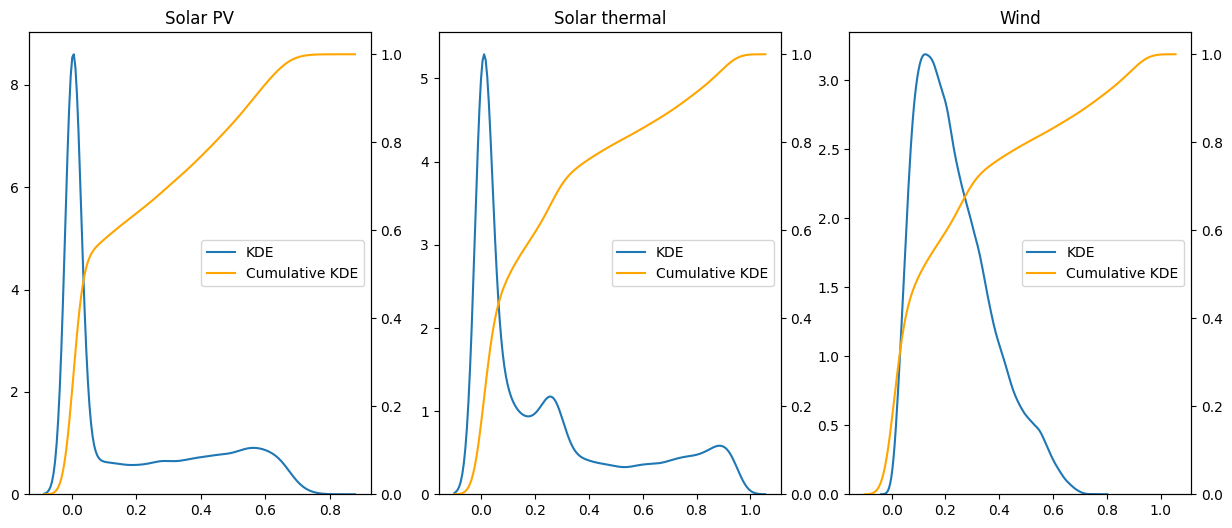
\includegraphics[width=\linewidth]{assets/kde-triple.png}
    \caption{KDE and cumulative KDE of the three capacity factors}
    \label{fig:kde-triple}
\end{figure}

Several observations can be made regarding these plots. First of all, the high density of zero like values in both solar plots is clear, with an even higher denisty in the solar PV. In fact it can be seen how both KDE have non zero values for x values below zero, however this only happens due to the symmetry and width of the gaussian kernel, which for the points at zero sums some value for points below zero. Appart from the mode at zero, both plots have another peak near their maximum value, at around 0.6 and 0.9 for the solar PV and solar thermal respectively. This is due to the shape of the solar ecliptic, where the sun remains at its highest point for longer than it is at any given point during ascent or descent. The solar thermal PDF also has a significant peak at around 0.3, probably due to this being the power at which the power plants runs with the stored heat at night. This is in fact the point where the daily curve in \autoref{fig:st-year-day} can be seen operating at night. As for the wind PDF and CDF, it is a much smoother plot, with the mode around 0.1 and then slowly and gradually tapers of. 

In order to have a more quantitative view of these distributions, metrics relating to the first four moments are shown in \autoref{table:main-moments}

\begin{table}[ht]
    \centering
    \begin{tabular}{rccc}
        \toprule
        Metric & \multicolumn{3}{c}{Value} \\ 
        \cmidrule(lr){2-4}
            & Solar PV & Solar Thermal & Wind \\
        \midrule
        Mean & 0.18 & 0.24 & 0.23 \\
        Standard Deviation & 0.23 & 0.29 & 0.14 \\
        Skew & 0.88 & 1.12 & 0.78 \\
        Kurtosis & -0.79 & -0.08 & 0.01 \\
        \bottomrule
    \end{tabular}
    \caption{Main moments of the three capacity factors}
    \label{table:main-moments}
\end{table}

Through these measures it can be seen how some of the intuitions obtained when looking at the time series plot of the different capacity factors were wrong. For example, the wind capacity factor is not the most volatile as it seemed, but in fact has the lowest standard deviation. This could be however due to the high variability of the solar profile, and taking away the seasonality of the three variables these metrics could be different.

\subsubsection{Lagged relationships}
Another key factor about the three series is their seasonality and how a given value at $t$ is influenced by past values at $t-1, t-2...$. In order to explore these relationships, two different metrics will be used. 

The first one is the the autocorrelation. While correlation as expressed by the Pearson correlation coefficient is generally calculated like
\begin{equation}
    \rho{\left(X,Y\right)}=\frac{\text{cov}\left(X,Y\right)}{\sigma_X\sigma_Y}=\frac{\sum^n_{i=1}\left(x_i-\bar{x}\right)\left(y_i-\bar{y}\right)}{\sqrt{\sum^n_{i=1}\left(x_i-\bar{x}\right)^2}\sqrt{\sum^n_{i=1}\left(y_i-\bar{y}\right)^2}}
\end{equation} 

The autocorrelation function of a series quantifies the correlation of a series with lagged values of itself at different lags. For a given lag $k$ it is thus calculated like
\begin{equation}
    \label{eq:acf}
    ACF\left(k\right)=\frac{\sum^{N-k}_{t=1}\left(x_t-\bar{x}\right)\left(x_{t+k}-\bar{x}\right)}{\sum^{N}_{t=1}\left(x_t-\bar{x}\right)^2}
\end{equation} 

The correlation coefficient has some known drawbacks however. It only measures linear relationships, so any dependence appart from this very simple relationship cannot be captured through a high correlation coefficient. That is what the new correlation coefficient proposed by \cite{correlation_2021} aims to solve, and why it has been included here. This new correlation coefficient, capable of capturing non linear relationships and with some very interesting statistical properties is calculated as 
\begin{equation}
    \xi{\left(X,Y\right)}=1-\frac{3\sum_{i=1}^{n-1}\left|r_{i+1}-r_i\right|}{n^2-1}
\end{equation}

Where the given pairs $\left(x_1,y_1\right), \left(x_2,y_2\right)...\left(x_n,y_n\right)$ have been aranged so that $x_1 \leq...\leq x_n$. Here $r_i$ denotes the rank of $y_i$. That is, the number of $j$ such that $y_j\leq y_i$. If there are ties among the $x$ values, the formula is slightly different, however with the capacity factor being a continuous variable it can be assumed that no ties will be present. Finally, note how even though $\rho \in \left[-1,1\right]$ the new correlation coefficient makes no distinction between positive and negative relationships and $\xi \in \left[0,1\right]$.

With this new correlation coefficient, a new autocorrelation function is constructed in the same way as in \eqref{eq:acf}, calculating the correlation of the series with its lagged values for each lag. The following figure shows both autocorrelation functions for the three series. 

\begin{figure}[ht]
    \centering
    \captionsetup{justification=centering}
    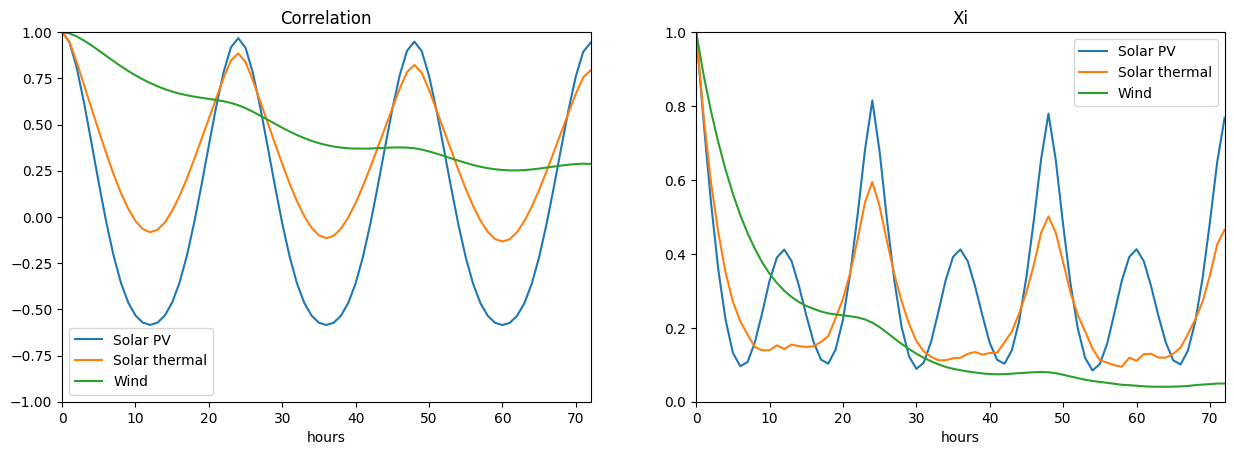
\includegraphics[width=\linewidth]{assets/autocorrelation.png}
    \caption{Autocorrelation functions with the two correlation coefficients for the three capacity factors at different hourly lags}
    \label{fig:autocorrelation}
\end{figure}

Several observations can be made from the two autocorrelation functions in \autoref{fig:autocorrelation}. The seasonality in both solar series is again made apparent, with high autocorrelations at the 24, 48 and 72 hour mark showcasing the importance of the previous days' values at the same hour for a given day, but also at the 12, 36 and 60 hour mark. This second autocorrelation, negative in the case of pearson correlation, denotes the relationship between opposite moments of the day between different days. It is also noted how the correlation in the case of the solar PV is much more persistent, with the correlation peaks remaining more or less constant for the three days, while for the solar thermal this correlation tapers off a little bit faster. It is also interesting to see how the correlation at the 12, 36 and 60 hour mark is a lot lower for the solar thermal, showcasing how this relatinoship between values at a lag of 12 hours practically -- although not completely -- disappears, again due to the inertia of the thermal system which makes the solar thermal cycle less related to the sun's trayectory. As for the wind autocorrelation functions, it is much more linear and smooth, with the relevance of past values reducing gradually as the hours go by. There is a slight daily seasonality as well with the autocorrealtion at daily lags being slightly above what could be expected from the linear trend. However, this has a practically negligible relevance compared with the solar series. In fact, for the wind capacity factor it can be seen how the immediately previous values have much higher significance, while previous lags at the daily or semidaily periods hold much less significance. 

\textcolor{red}{INCLUDE SEASONAL LAGS?}
\subsubsection{Seasonal statistical characteristics}
Even though the characteristics shown in previous sections already provides very significant information, it seems like many of these characteristics may be seasonally dependent. That is, they may not be the same in summer and in winter, or at night and during the day. That is why the previous analyses will be performed again but seasonally separating the datasets. Both daily and yearly splits will be done, where "day" is the period from 06:00 to 18:00 UTC and "night" is the period from 18:00 to 06:00 UTC. On the yearly split and taking into account the day's number within a year, spring goes from the 3\textsuperscript{rd} to the 5\textsuperscript{th} month, summer from the 6\textsuperscript{th} to the 8\textsuperscript{th}, autoumn from the 9\textsuperscript{th} to the 11\textsuperscript{th} and winter from the 12\textsuperscript{th} to the 2\textsuperscript{nd}, both inclusive in all cases. Note how these are metereological seasons, and not astronomical seasons based on the solstices and equinoxes. 

The yearly seasonal breakdown can be seen in \autoref{fig:kde-triple-seasonal}. 

\begin{figure}[ht]
    \centering
    \captionsetup{justification=centering}
    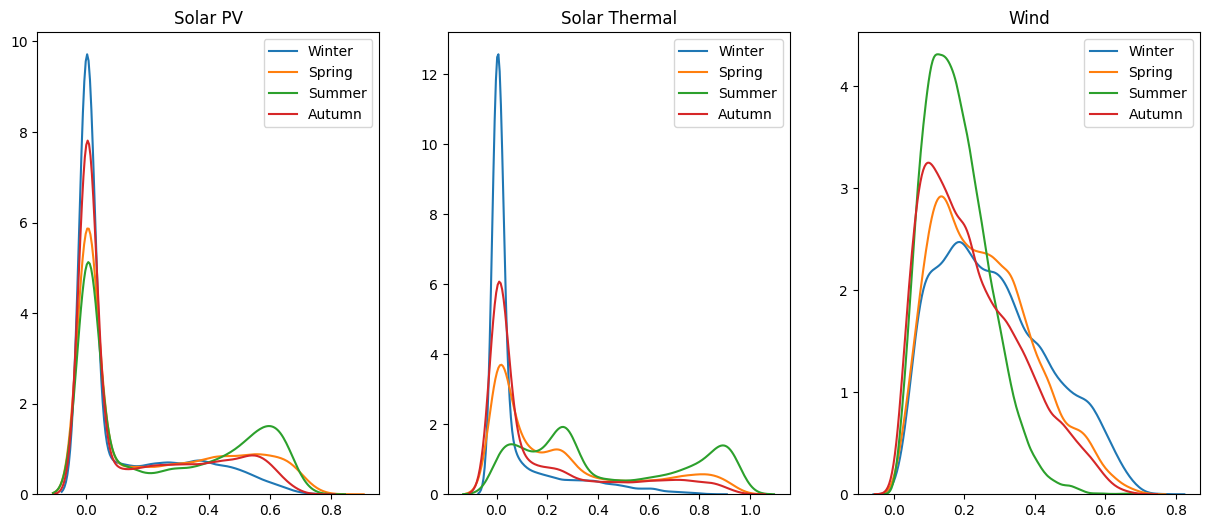
\includegraphics[width=\linewidth]{assets/kde-triple-seasonal.png}
    \caption{KDE plot for the three capacity factors for the different yearly seasons}
    \label{fig:kde-triple-seasonal}
\end{figure}

For the solar PV it can be seen how on one extreme in winter the concentration of zeroes is highest, with very low density in the previously seen peak at 0.6, while in the summer the concentration of zeroes is still high -- due to the night hours -- but much less, and the peak at 0.6 can be clearly seen. Spring and autumn are found in between these values, with spring having a density of zeroes slightly above summer but a much lower peak at 0.6. For solar thermal the difference in density at zero is much higher, with winter having higher density and the rest of the seasons having a much lower one. In fact, for summer density at zero es very low, much more than other peaks. The peak at 0.9 can again only be seen in the summer, and the peak at 0.3 can be seen mainly for summer but also slightly for spring. As for the wind distribution, the summer season seems to be the one with the lowest volatility and lowest mean, while winter has the widest PDF and apparently mean.  

\begin{figure}[ht]
    \centering
    \captionsetup{justification=centering}
    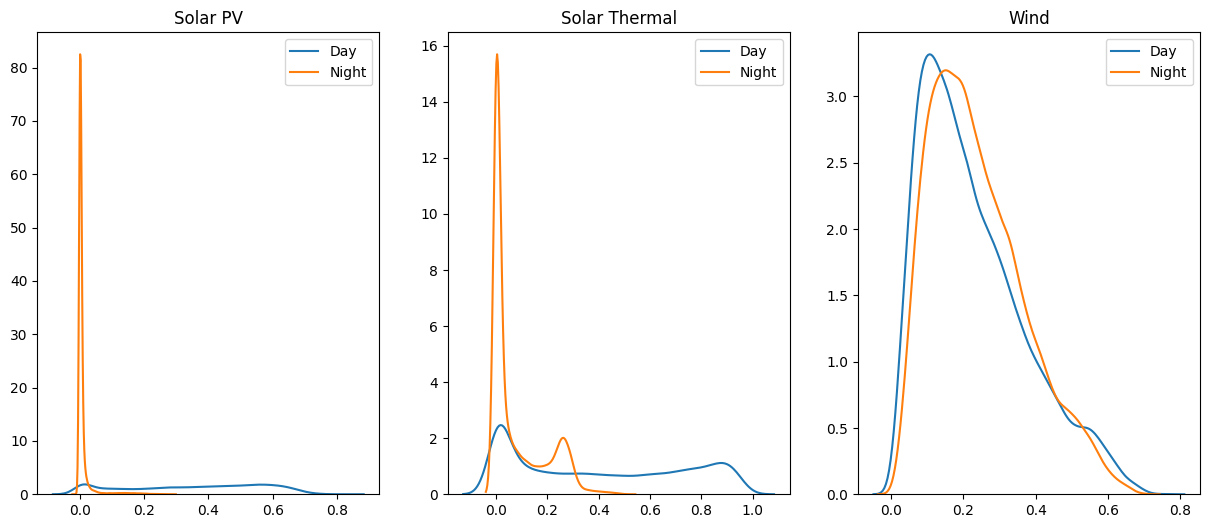
\includegraphics[width=\linewidth]{assets/kde-triple-daily.png}
    \caption{KDE plot for the three capacity factors for the different daily periods}
    \label{fig:kde-triple-daily}
\end{figure}

In \autoref{fig:kde-triple-daily} a similar representation for the KDE can be seen but for the split between night and day. For solar PV the plot is not very interesting, with the night having all its density at the zero point, with the day density having a slight peak at zero -- as the exact times for sunset and sunrise vary during the year and the period defined here as "day" can in fact have some night time -- and the already known one at 0.6. For solar thermal it can be seen how the peak at 0.9 is exclusively a day time fenomenon while the peak at 0.3 is a night time fenomenon, confirming the hypothesis that this was the power generated at night with the stored heat from the day. For the wind, it can be seen how the difference between day and night is practically negligible, with day exhibiting a slightly more "summer" like behaviour -- that is, slightly less volatile and lower mean. 

\subsubsection{Multivariate analysis}
Up until this point every analysis has been performed on a per variable basis, examining their individual properties. However, when thinking about the true implications for the power grid it becomes clear that the joint characteristics are also fundamental. For a given wind and solar distributions, the consequences of the grid are not the same if peaks in both happen at the same time or if they complement each other. That is why the joint characteristics will be studied, and they will mainly be studied through cross correlation and through copula analysis. Some other analysis, like through Granger causality as outlined in \cite{granger_1969} were attempted, but no new relevant information that wasn't uncovered through cross correlation was found. 

Cross correlation follows a principle very similar to the autocorrelation, but instead of measuring the correlation of a series with lagged versions of itself, the correlation of a variable with lagged versions of a different variable are measured. That way, something similar to the predictive value of the second variable on the first can be understood. Again, the two different correlation coefficients already explained were used. Note how for Person's correlation the relationship for $\left(X,Y\right)$ is the same as for $\left(Y,X\right)$. However, when using lagged values the correlation does depend on which variable is lagged. for the new correlation coefficient the directionality matters, as the effect of one variable on a second is not the same as that of the second on the first one. 

In \autoref{fig:cross-correlation} the lagged cross correlation between each pair of variables can be seen. For each of the three variables, it is shown how the lagged versions of the other two are correlated to the given variable, for each of the two correlation coefficients. 

\begin{figure}[ht]
    \centering
    \captionsetup{justification=centering}
    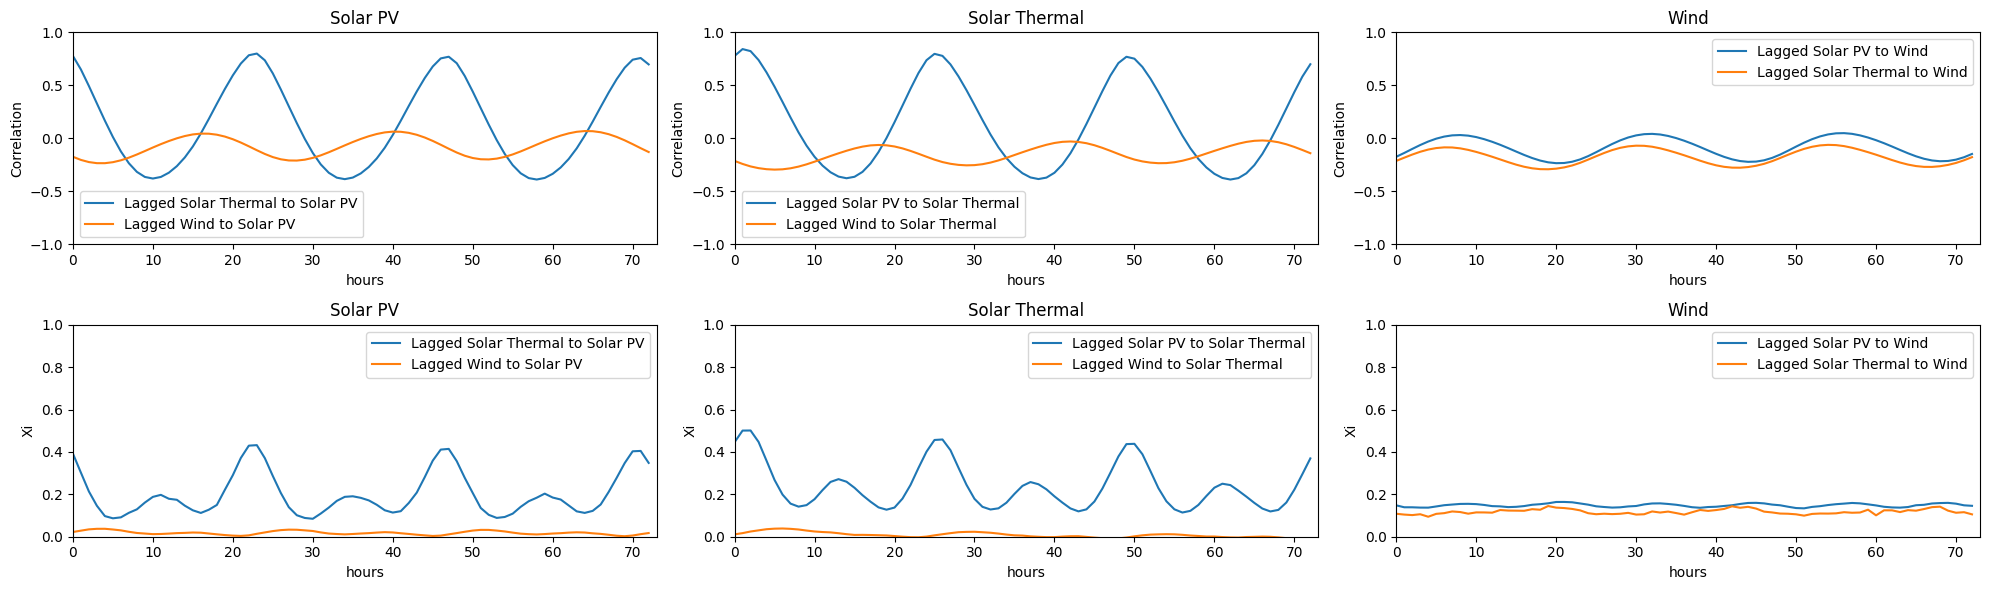
\includegraphics[width=\linewidth]{assets/cross-correlation.png}
    \caption{Lagged cross correlation between each pair of capacity factors}
    \label{fig:cross-correlation}
\end{figure}

The similarity between the solar PV and solar thermal is clearly shown, with high correlations in both directions. Interestingly, the solar thermal capacity factor is more highly correlated with the 1-lag solar PV than with the simultaneous solar PV, probably due to the time it takes for the working fluid to be heated up, while the PV cells are able to convert that sunlight into power instantaneously. The second notable observation is that the predictive power of solar on wind seems to be higher than that of wind on any solar when looking at the Xi. Also, that correlation of the two lagged solar variables does not seem to decay for the examined 3 day period, and a very slight lag effect is seen where the daily seasonality of the sunlight is seen in the correlation, with wind being negatively correlated to simultaneous solar power but positively correlated to solar power at a lag of around 8 hours. 

\textcolor{red}{INCLUDE SEASONAL CROSS LAGS?}

The second method used to see how the three variables compare to each other will be using copulas. Copulas are multivariate functions used to model the dependence between several random variables. Consider the random vector $(X_1,X_2,X_3)$ representing the observations of capacity factor for solar PV, solar thermal and wind energy for a given point in time. The marginal CDF of each of the variables is represented as $F_i\left(x\right)=p\left(X_i\leq x\right)$, which when applied to the random vector yields the marginals $\left(U_1,U_2,U_3\right)=\left(F_1\left(X_1\right),F_2\left(X_2\right),F_3\left(X_3\right)\right)\in \left[0,1\right]^3$. The copula $C(\cdot)$ is the joint cumulative distribution function such that 
\begin{equation}
    C\left(u_1,u_2,u_3\right)=p\left(U_1\leq u_1,U_2\leq u_2,U_3\leq u_3\right)
\end{equation}

The copula contains all information on the dependence structure between the three series, while the marginal cumulative distribution functions contain all inforamtion on the marginal distribution of the variables. 

In this analysis, the marginal CDF used has been the gaussian cumulative KDE outlined in \eqref{eq:cumulative-kde}. The copula used has been a gaussian copula, which relies on the multivariate normal distribution.

For the fitting process, a cumulative gaussian KDE is fitted for each of the variables and then the univariate values are transformed according to that CDF. Then, the normal percent point function (PPF) -- the inverse of the CDF -- is applied to transformed variable to normalize it. Then, a multivariate gaussian is fitted on the normalized data. 

The correlation matrix of the gaussian copula can be seen in \autoref{table:copula-correlation-matrix}.

\begin{table}[ht]
    \centering
    \begin{tabular}{r|ccc}
        & Solar PV & Solar thermal & Wind \\
        \midrule
        Solar PV & 1.00 & 0.72 & -0.19 \\
        Solar thermal & 0.72 & 1.00 & -0.23 \\
        Wind & -0.19 & -0.23 & 1.00 \\
    \end{tabular}
    \caption{Correlation matrix of the gaussian copula with gaussian KDE marginals}
    \label{table:copula-correlation-matrix}
\end{table}

It can be seen how in the copula representation the strong positive correlation between both solar series and the negative correlation between wind and both solar series still stands. 